
\de{ĐỀ THI HỌC KỲ I NĂM HỌC 2022-2023}{THPT Mạc Đỉnh Chi}
\begin{center}
	\textbf{PHẦN 1 - TRẮC NGHIỆM}
\end{center}
\Opensolutionfile{ans}[ans/ans]
\begin{ex}%[0T1Y1-1]%[Dự án đề kiểm tra HKII NH22-23- Nguyễn Văn Sang ]%[THPT Mạc Đỉnh Chi]
Trong các câu sau, câu nào không phải là mệnh đề?
\choice
{$\sqrt{2}$ là số vô tỉ}
{$3^2+4^2=5^2$}
{$\exists x \in \mathbb{N}, x+1=0$}
{\True Mấy giờ rồi?}
\loigiai{
``Mấy giờ rồi?'' là một câu hỏi, không phải là mệnh đề vì \textbf{mệnh đề} là một khẳng định đúng hoặc sai.
}
\end{ex}
\begin{ex}%[0T1Y1-3]%[Dự án đề kiểm tra HKII NH22-23- Nguyễn Văn Sang ]%[THPT Mạc Đỉnh Chi]
Mệnh đề phủ định của mệnh đề $P\colon ``\forall x \in \mathbb{R}, x^2+x+1>0''$ là
\choice
{$\overline{P}\colon `` \exists x \in \mathbb{R}, x^2+x+1>0 ''$}
{\True $\overline{P}\colon `` \exists x \in \mathbb{R}, x^2+x+1 \leq 0 ''$}
{$\overline{P}\colon `` \exists x \in \mathbb{R}, x^2+x+1 \geq 0 ''$}
{$\overline{P}\colon `` \exists x \in \mathbb{R}, x^2+x+1=0 ''$}
\loigiai{
 Phủ định của mệnh đề $P\colon ``\forall x \in \mathbb{R}, x^2+x+1>0''$ là $\overline{P}\colon `` \exists x \in \mathbb{R}, x^2+x+1 \leq 0 ''$.
}
\end{ex}
\begin{ex}%[0T1Y2-1]%[Dự án đề kiểm tra HKII NH22-23- Nguyễn Văn Sang ]%[THPT Mạc Đỉnh Chi]
Hãy viết lại tập hợp $A=\{x \in \mathbb{N} \mid x<5\}$ dưới dạng liệt kê các phần tử.
\choice
{\True $A=\{0;1;2;3;4\}$}
{$A=\{0;1;2;3;4;5\}$}
{$A=\{1;2;3;4;5\}$}
{$A=\{1;2;3;4\}$}
\loigiai{
Tập hợp $A=\{x \in \mathbb{N} \mid x<5\}$ viết lại dưới dạng liệt kê các phần tử là $A=\{0;1;2;3;4\}$.
}
\end{ex}
\begin{ex}%[0T2Y1-2]%[Dự án đề kiểm tra HKII NH22-23- Nguyễn Văn Sang ]%[THPT Mạc Đỉnh Chi]
Cặp số nào sau đây là nghiệm của bất phương trình $x+2y>0$?
\choice
{$(0;0)$}
{$(1,-1)$}
{\True $(-1;2)$}
{$(-2;1)$}
\loigiai{
Xét bất phương trình $x+2y>0$.\\
Ta có $(-1)+2\cdot2=3>0$ nên $(-1;2)$ là nghiệm của bất phương trình $x+2y>0$.
}
\end{ex}
\begin{ex}%[0T2Y2-1]%[Dự án đề kiểm tra HKII NH22-23- Nguyễn Văn Sang ]%[THPT Mạc Đỉnh Chi]
Hệ bất phương trình nào sau đây là hệ bất phương trình bậc nhất hai ẩn?
\choice
{$\heva{&x+y^2>1 \\& 2x-y<3}$}
{$\heva{&x+3y>x y \\& 2x-y<5}$}
{$\heva{&x+x y>3 \\& x-2x<x^2}$}
{\True $\heva{&x+2y>1 \\& x-y<0}$}
\loigiai{
Ta có $\heva{&x+2y>1 \\& x-y<0}$ là hệ bất phương trình bậc nhất hai ẩn.
}
\end{ex}
\begin{ex}%[0T3Y1-2]%[Dự án đề kiểm tra HKII NH22-23- Nguyễn Văn Sang ]%[THPT Mạc Đỉnh Chi]
Tập xác định $\mathscr{D}$ của hàm số $y=f(x)=\dfrac{|x|}{x+5}$ là
\choice
{$\mathscr{D}=(-5;+\infty)$}
{$\mathscr{D}=(-\infty;5)$}
{$\mathscr{D}=\mathbb{R}$}
{\True $\mathscr{D}=\mathbb{R}\setminus \{-5\}$}
\loigiai{
Hàm số có nghĩa khi $x+5\neq 0\Leftrightarrow x\neq -5$.\\
Vậy tập xác định $\mathscr{D}=\mathbb{R}\setminus \{-5\}$.
}
\end{ex}
\begin{ex}%[0T3Y2-3]%[Dự án đề kiểm tra HKII NH22-23- Nguyễn Văn Sang ]%[THPT Mạc Đỉnh Chi]
Trục đối xứng của parabol $(P)\colon y=x^2+4x-2$ là đường thẳng có phương trình là
\choice
{$x=2$}
{\True $x=-2$}
{$y=2$}
{$y=-2$}
\loigiai{
	Đồ thị hàm số bậc hai $y=ax^2+bx+c$ (với $a\ne 0$) là một parabol có trục đối xứng là đường thẳng $x=-\dfrac{b}{2}$.\\
	Áp dụng  parabol $(P)\colon y=x^2+4x-2$ có trục đối xứng là đường thẳng $x=-\dfrac{4}{2\cdot1}=-2$.
}
\end{ex}
\begin{ex}%[0T4Y1-1]%[Dự án đề kiểm tra HKII NH22-23- Nguyễn Văn Sang ]%[THPT Mạc Đỉnh Chi]
Cho $90^{\circ}<x<180^{\circ}$. Khẳng định nào sau đây là \textbf{sai}?
\choice
{$\sin x>0$}
{\True $\tan x>0$}
{$\cos x<0$}
{$\cot x<0$}
\loigiai{
Với điều kiện $90^{\circ}<x<180^{\circ}$ thì $\sin x>0$, $\cos x<0$ suy ra $\tan x=\dfrac{\sin x}{\cos x}>0$ là sai.
}
\end{ex}
\begin{ex}%[0T4Y2-1]%[Dự án đề kiểm tra HKII NH22-23- Nguyễn Văn Sang ]%[THPT Mạc Đỉnh Chi]
Cho tam giác $ABC$ có $AB=5$, $AC=7$ và $BC=8$. Tính $\cos A$.
\choice
{$\dfrac{1}{8}$}
{$\dfrac{1}{5}$}
{\True $\dfrac{1}{7}$}
{$\dfrac{7}{8}$}
\loigiai{
\immini
{
Áp dụng định lý cosin trong tam giác $ABC$ ta có
 $$\cos A=\dfrac{AB^2+AC^2-BC^2}{2\cdot AB \cdot AC}=\dfrac{5^2+7^2-8^2}{2\cdot 5 \cdot 7}=\dfrac{1}{7}.$$
}
{
\begin{tikzpicture}[line join = round, line cap = round,>=stealth,thick,font=\footnotesize,scale=.75]
	\fill (0,4) coordinate (A) circle (1pt) node[above]{$A$};
	\fill (-2,0)coordinate (B) circle (1pt) node[below]{$B$};
	\fill (4,0)coordinate (C) circle (1pt) node[below]{$C$};
	\draw (A)--(B)--(C)--cycle;
	\draw pic[draw,blue,angle radius=3mm,angle eccentricity=1.5] {angle =B--A--C}; 
\end{tikzpicture}
}
}
\end{ex}
\begin{ex}%[0T4Y1-3]%[Dự án đề kiểm tra HKII NH22-23- Nguyễn Văn Sang ]%[THPT Mạc Đỉnh Chi]
Khẳng định nào sau đây luôn đúng với mọi giá trị $x$ làm cho biểu thức có nghĩa?
\choice
{$\cot ^2x+\tan ^2x=1$}
{$\dfrac{1}{\sin ^2x}=1+\tan ^2x$}
{$\sin ^2x-\cos ^2x=1$}
{$\dfrac{1}{\cos ^2x}=1+\tan ^2x$}
\loigiai{
 Với mọi giá trị $x$ làm cho biểu thức có nghĩa thì biểu thức $\dfrac{1}{\cos ^2x}=1+\tan ^2x$ là đúng.
}
\end{ex}



%%%% Câu 11
\begin{ex}%[0T5Y1-1]%[Dự án đề kiểm tra HKI NH22-23- Thành Đức Trung]%[THPT Mạc Đĩnh Chi - Hồ Chí Minh]
	Cho ba điểm $A$, $B$, $C$. Có bao nhiêu véc-tơ khác véc-tơ không có điểm đầu và điểm cuối là các điểm đã cho.
	\choice
	{3}
	{4}
	{5}
	{\True 6}
	\loigiai
	{Các véc-tơ khác véc-tơ không có điểm đầu và điểm cuối trong ba điểm $A$, $B$, $C$ là: $\overrightarrow{AB}$, $\overrightarrow{BA}$, $\overrightarrow{AC}$, $\overrightarrow{CA}$, $\overrightarrow{BC}$ và $\overrightarrow{CB}$.\\
		Vậy có 6 véc-tơ thỏa mãn yêu cầu bài toán.		
	}
\end{ex}

%%%% Câu 12
\begin{ex}%[0T5Y2-1]%[Dự án đề kiểm tra HKI NH22-23- Thành Đức Trung]%[THPT Mạc Đĩnh Chi - Hồ Chí Minh]
	Cho hình bình hành $ ABCD $. Khẳng định nào sau đây là đúng?
	\choice
	{\True $\overrightarrow{AB}+\overrightarrow{AD}=\overrightarrow{AC}$}
	{$\overrightarrow{AB}+\overrightarrow{BC}=\overrightarrow{CA}$}
	{$\left|\overrightarrow{BD}\right|=\left|\overrightarrow{AC}\right|$}
	{$\left|\overrightarrow{AD}\right|=\left|\overrightarrow{AB}\right|$}
	\loigiai
	{Do $ ABCD $ là hình bình hành nên theo quy tắc hình bình hành ta có $\overrightarrow{AB}+\overrightarrow{AD}=\overrightarrow{AC}$.
	}
\end{ex}

%%%% Câu 13
\begin{ex}%[0T3Y1-4]%[Dự án đề kiểm tra HKI NH22-23- Thành Đức Trung]%[THPT Mạc Đĩnh Chi - Hồ Chí Minh]
	Đồ thị hàm số $y=x^2+x+1$ đi qua điểm nào sau đây?
	\choice
	{$M(0;-1)$}
	{$N(2;5)$}
	{\True $P(1;3)$}
	{$Q(-2;-5)$}
	\loigiai
	{Do $3=1^2+1+1$ nên đồ thị hàm số $y=x^2+x+1$ đi qua điểm $P(1;3)$.
	}
\end{ex}

%%%% Câu 14
\begin{ex}%[0T5B4-1]%[Dự án đề kiểm tra HKI NH22-23- Thành Đức Trung]%[THPT Mạc Đĩnh Chi - Hồ Chí Minh]
	Cho tam giác đều $ABC$ cạnh bằng 2. Tính $\overrightarrow{AB}\cdot\overrightarrow{AC}$.
	\choice
	{4}
	{3}
	{\True 2}
	{1}
	\loigiai
	{Do tam giác $ ABC $ đều nên $\left(\overrightarrow{AB},\overrightarrow{AC}\right)=\widehat{BAC}=60^{\circ}$.\\
		Ta có \[\overrightarrow{AB}\cdot\overrightarrow{AC}=\left|\overrightarrow{AB}\right|\cdot\left|\overrightarrow{AC}\right|\cdot\cos\left(\overrightarrow{AB},\overrightarrow{AC}\right)=2\cdot2\cdot\cos60^{\circ}=2.\]
		Vậy $\overrightarrow{AB}\cdot\overrightarrow{AC}=2$.	
	}
\end{ex}

	%%%% Câu 15
	\begin{ex}%[0T6Y3-1]%[Dự án đề kiểm tra HKI NH22-23- Thành Đức Trung]%[THPT Mạc Đĩnh Chi - Hồ Chí Minh]
		Tìm số trung bình của mẫu số liệu sau: $3; 5; 7; 8; 12; 14; 20; 25; 30; 32$
		\choice
		{$15{,}5$}
		{\True $15{,}6$}
		{$15{,}7$}
		{$15{,}8$}
		\loigiai
		{Số trung bình của mẫu số liệu trên là $\overline{x}=\dfrac{3+5+7+8+12+14+20+25+30+32}{10}=15{,}6$.
			
		}
	\end{ex}
	
	%%%% Câu 16
	\begin{ex}%[0T6Y1-2]%[Dự án đề kiểm tra HKI NH22-23- Thành Đức Trung]%[THPT Mạc Đĩnh Chi - Hồ Chí Minh]
		Quy tròn số $7216{,}47$ đến hàng chục ta được số nào sau đây?
		\choice
		{$7200$}
		{\True $7220$}
		{$7210$}
		{$7216{,}5$}
		\loigiai
		{Vì chữ số sau hàng quy tròn lớn hơn $5$ nên số quy tròn của số trên là $7220$.
		}
	\end{ex}
	
	%%%% Câu 17
	\begin{ex}%[0T6Y3-3]%[Dự án đề kiểm tra HKI NH22-23- Thành Đức Trung]%[THPT Mạc Đĩnh Chi - Hồ Chí Minh]
		Điểm đánh giá định kỳ môn Toán của $45$ học sinh lớp $10A$ được cho bởi bảng sau
		\begin{center}
			\begin{tabular}{|l|c|c|c|c|c|c|c|l|}
				\hline Điểm & $6$ & $6,5$ & $7$ & $7,5$ & $8$ & $8,5$ & $9$ & $10$ \\
				\hline Số học sinh & $4$ & $3$ & $3$ & $5$ & $10$ & $15$ & $3$ & $2$\\
				\hline
			\end{tabular}
		\end{center}
		Mốt của mẫu số liệu trên là
		\choice
		{$10$}
		{\True $15$}
		{$8$}
		{$8{,}5$}
		\loigiai
		{Vì điểm $8{,}5$ có số học sinh đạt nhiều nhất nên mốt của mẫu số liệu trên là $M_O=15$.
		}
	\end{ex}

%%%% Câu 18
\begin{ex}%[0T1B3-4]%[Dự án đề kiểm tra HKI NH22-23- Thành Đức Trung]%[THPT Mạc Đĩnh Chi - Hồ Chí Minh]
	Cho hai tập hợp $A = \left\{1;2;3;4;5\right\}$ và $B = \left\{x\in\mathbb{N}\Big|\left(x-1\right)\left(x^2-3x-4\right) = 0\right\}$. Khi đó tập hợp $A\cup B$ có bao nhiêu phần tử
	\choice
	{$7$}
	{\True $5$}
	{$8$}
	{$3$}
	\loigiai
	{
		Xét tập hợp $B$. Ta có \[\left(x-1\right)\left(x^2-3x-4\right) = 0 \Leftrightarrow\hoac{&x-1=0\\&x^2-3x-4=0}\Leftrightarrow \hoac{&x=1\\&\hoac{&x=-1\quad\left(\text{loại}\right)\\&x=4.}}\]
		Do đó $B = \left\{1;4\right\}$. Suy ra $A\cup B = \left\{1;2;3;4;5\right\}$ có $5$ phần tử.
	}
\end{ex}

%%%% Câu 19
\begin{ex}%[0T1B3-5]%[Dự án đề kiểm tra HKI NH22-23- Thành Đức Trung]%[THPT Mạc Đĩnh Chi - Hồ Chí Minh]
	Cho ba tập hợp $A = \left[5;9\right]$, $B = \left(6;10\right]$ và $C = \left(3;8\right]$. Tìm $C\backslash\left(A\cap B\right)$.
	\choice
	{$\left(3;6\right)$}
	{\True $\left(3;6\right]$}
	{$\left(3;5\right)$}
	{$\left(3;5\right]$}
	\loigiai
	{
		Ta có $A\cap B = \left(6;9\right]$. Suy ra $C\backslash\left(A\cap B\right) = \left(3;6\right]$.
	}
\end{ex}

%%%% Câu 20
\begin{ex}%[0T2B2-2]%[Dự án đề kiểm tra HKI NH22-23- Thành Đức Trung]%[THPT Mạc Đĩnh Chi - Hồ Chí Minh]
	\immini{ Miền không bị gạch chéo (như hình vẽ) là miền nghiệm của bất phương trình nào sau đây?
		\choice
		{\True $2x+y>2$}
		{$2x+y<2$}
		{$x+2y>2$}
		{$x+2y<2$}
	}{
		\begin{tikzpicture}[line join=round, line cap=round, >=stealth,font=\footnotesize, scale=0.7]
			\draw[->](-5,0)--(4,0) node[below right] {$x$};
			\draw[->](0,-3)--(0,5) node[left] {$y$};
			\clip (-5,-3) rectangle (4,5);
			\node (0,0) [below left]{$ O $};
			\foreach \x in {-4,...,3}
			\draw[shift={(\x,0)},color=black] (0pt,2pt) -- (0pt,-2pt);
			\foreach \y in {-2,...,4}
			\draw[shift={(0,\y)},color=black] (2pt,0pt) -- (-2pt,0pt);
			\draw[samples=100,smooth,domain=-3:5] plot(\x,{-2*(\x)+2});
			\draw [pattern=dots] (-5,5)--(-1.5,5)--(2.5,-3)--(-5,-3)--cycle;
			\draw[fill=black] (1,0) circle(1pt) node[above]{$1$};
			\draw[fill=black] (0,2) circle(1pt) node[right]{$2$};
		\end{tikzpicture}
	}	
	\loigiai
	{
		Điểm $\left(0;0\right)$ \textbf{không} thuộc miền nghiệm nên ta loại đáp án \lq\lq $2x+y<2$\rq\rq\; và \lq\lq$x+2y<2$\rq\rq.\\
		Điểm $\left(2;0\right)$ thuộc miền nghiệm nên ta loại đáp án \lq\lq$x+2y<2$\rq\rq.
	}
\end{ex}

%%==========Câu 21
\begin{ex}%[0D4B4-3]
Bác An dự định để $x$ sào đất trồng cà tím và $y$ sào đất trồng cà chua. Bác dự định để tối đa $10$ triệu đồng để mua hạt giống. Tiền mua hạt giống cà tím là $200.000$ đồng/sào và cà chua là $100.000$ đồng/sào. Hệ bất phương trình mô tả điều kiện của $x$, $y$ là
\choice
{$\heva{&2x+y\geq 100\\ &x\geq 0\\ &y\geq 0}$}
{$\heva{&2x+y\leq 1000\\ &x\geq 0\\ &y\geq 0}$}
{\True $\heva{&2x+y\leq 100\\ &x\geq 0\\ &y\geq 0}$}
{$\heva{&x+2y\leq 100\\ &x\geq 0\\ &y\geq 0}$}
\loigiai{
Theo đề bài thì điều kiện của $ x $ và $ y $ thoả mãn hệ phương trình
$$
	\heva{&200\,000 x+100\,000 y\leq 10\,000\,000\\ &x\geq 0\\ &y\geq 0}
	\Leftrightarrow
	\heva{&2x+y\leq 100\\ &x\geq 0\\ &y\geq 0.}
$$
}
\end{ex}
%%==========Câu 22
\begin{ex}%[0D2B1-1]
Cho hàm số $y=f(x)=\heva{&\sqrt{x+1}\quad\text{khi}~x\geq-1\\ &x^2-x-1\quad\text{khi}~-5\leq x<-1}$. Tính $f(0)+f(-2)$
\choice
{$0$}
{$2$}
{$4$}
{\True $6$}
\loigiai{
Có: $f(0)=1$, $f(-2)=5$. Vậy $f(0)+f(-2)=6$.
}
\end{ex}
%%==========Câu 23
\begin{ex}%[0H1B2-5]
Cho hình chữ nhật $ABCD$ có $AB=3$, $AD=4$. Tính $|\overrightarrow{A B}+\overrightarrow{A D}|$.
\choice
{$7$}
{$6$}
{\True $5$}
{$4$}
\loigiai{
Theo định lý Pytago: $BD=AC=\sqrt{AB^2+AD^2}=5$.\\
Có: $|\overrightarrow{A B}+\overrightarrow{A D}|=|\vec{AC}|=5$.
}
\end{ex}
%%==========Câu 24
\begin{ex}%[0D2B3-2]
\immini{Cho hàm số $y=a x^2+b x+c(a\ne 0)$ có đồ thị như hình vẽ bên. Khẳng định nào sau đây là đúng?}{\begin{tikzpicture}[x=1cm,y=1cm,scale=.6,>=stealth]
\def\aa{1/4} \def\bb{1} \def\cc{-1}
\draw[->] (-5.57,0)--(1.57,0)node[below right]{$x$};
\draw[->] (0,-3)--(0,1)node[left]{$y$};
\fill (0,0)node[below left]{$O$};
\draw[black,samples=150,smooth,domain=-5.47:1.47] plot(\x,{\aa*(\x)^2+\bb*\x+\cc});
\end{tikzpicture}
}
\choice
{$a>0,~b>0,~ c>0$}
{\True $a>0,~ b>0,~ c<0$}
{$a>0,~ b<0,~ c>0$}
{$a<0,~ b<0,~ c<0$}
\loigiai{
Đồ thị hàm số cắt trục tung tại điểm có tung độ âm, suy ra $c<0$.\\ Đồ thị có bề lõm hướng lên trên nên $a>0$.\\ Đỉnh của parabol $x=\dfrac{-b}{2a}<0\Rightarrow b>0$.
}
\end{ex}
%%==========Câu 25
\begin{ex}%[0D2B3-2]
Cho parabol $(P) \colon y=x^2+m x+n$. Tính $K=m-n$ biết $(P)$ cắt trục hoành tại hai điểm có hoành độ $1$ và $-5$
\choice
{\True $K=9$}
{$K=-1$}
{$K=1$}
{$K=-9$}
\loigiai{
Đồ thị hàm số cắt trục hoành tại hai điểm có hoành độ $1$ và $-5$ nên:\\
 $\heva{&1+m+n=0\\&25-5m+n=0}\Leftrightarrow \heva{&m=4\\&n=-5}$. Suy ra $m-n=9$.
}
\end{ex}
%%==========Câu 26
\begin{ex}%[0D2B3-1]
Hàm số $y=x^2-4x+3$ đồng biến trên khoảng nào sau đây?
\choice
{\True $(2;+\infty)$}
{$(-\infty;2)$}
{$(-2;+\infty)$}
{$(-\infty;+\infty)$}
\loigiai{
Đỉnh của parabol là $I(2;-1)$ và $ a=1>0 $\\
Vậy hàm số đồng biến trên khoảng $(2;+\infty)$.
}
\end{ex}
%%==========Câu 27
\begin{ex}%[0D2B3-2]
Biết parabol $(P): y=a x^2+b x+c$ đi qua hai điểm $A(1;2)$ và $B(-1;0)$. Tính $a+c$.
\choice
{$4$}
{$3$}
{$2$}
{\True $1$}
\loigiai{
Parabol $(P): y=a x^2+b x+c$ đi qua hai điểm $A(1;2)$ và $B(-1;0)$ nên:\\
$\heva{&a+b+c=2\\&a-b+c=0}\Leftrightarrow 2(a+c)=2 \Leftarrow a+c=1$.
}
\end{ex}
%%==========Câu 28
\begin{ex}%[0D6B3-4]
Cho tam giác $ABC$. Khẳng định nào sau đây là đúng
\choice
{$\sin (A+B)=-\sin C$}
{\True $\cos (A+B)=-\cos C$}
{$\tan (A+B)=\tan B$}
{$\cot (B+C)=\cot A$}
\loigiai{
Có: $A+B+C=180^{\circ} $. Suy ra $\sin (A+B)=\sin C$; $\cos (A+B)=-\cos C$.
}
\end{ex}
%%==========Câu 29
\begin{ex}%[0H2B3-1]
Cho tam giác $ABC$ biết $AB=AC=5$ và $BC=6$. Tính bán kính đường tròn nội tiếp tam giác $ABC$.
\choice
{$r=2$}
{$r=3$}
{$r=1$}
{\True $r=\dfrac{3}{2}$}
\loigiai{
Có $AB+AC+BC=16\Rightarrow p=\dfrac{AB+AC+BC}{2}=8$.\\
Diện tích tam giác $ABC$ là $S=\sqrt{p(p-AB)(p-AC)(p-BC)}=12$.\\
Có: $S=p\cdot r \Leftrightarrow r= \dfrac{S}{p}=\dfrac{12}{8}=\dfrac{3}{2}$.
}
\end{ex}
%%==========Câu 30
\begin{ex}%[0H1B2-2]
\immini{Cho hình bình hành $ABCD$. Gọi $I$ là trung điểm $CD$. Khẳng định nào sau đây là đúng ?}{\begin{tikzpicture}[scale=.6, font=\footnotesize,>=stealth]%<DTools>
%Gán tọa độ.
\coordinate (A) at (1,3);
\coordinate (B) at (0,0);
\coordinate (C) at (5,0);
\coordinate (D) at (6,3);
\coordinate (I) at (5.5,1.5);
%Vẽ tứ giác ABCD.
\draw (A)--(B)--(C)--(D)--cycle (A)--(I);
%Gán nhãn.
\foreach \x/\y in {I/0,A/90,B/-90,C/-90,D/90}{\fill (\x) circle(1pt) ($(\x)+(\y:0.3cm)$) node{$\x$};}
\end{tikzpicture}}
\choice
{$\vec{AI}=\vec{AB}+\dfrac{1}{2}\vec{AD}$}
{\True $\vec{AI}=\dfrac{1}{2}\vec{AB}+\vec{AD}$}
{$\vec{AI}=\vec{AB}-\dfrac{1}{2}\vec{AD}$}
{$\vec{AI}=-\dfrac{1}{2}\vec{AB}+\vec{AD}$}
\loigiai{
Có: $\vec{AI}=\vec{AD}+\vec{DI}=\vec{AD}+\dfrac{1}{2}\vec{DC}=\vec{AD}+\dfrac{1}{2}\vec{AB}$.
}
\end{ex}


%Câu 31...........................
\begin{ex}%%[0D6Y1-2]%[Dự án đề kiểm tra HKII NH22-23- Tên GV]%[Mạc Đĩnh Chi]
	Cho số gần đúng $a=23{,}471$ với độ chính xác $d=0{,}05$. Số quy tròn của số $a$ là
	\choice
	{\True $23{,}5$}
	{$23{,}4$}
	{$23$}
	{$23{,}47$}
	\loigiai{
		Hàng lớn nhất của độ chính xác $d=0{,}05$ là hàng phần trăm, nên ta quy tròn $a$ đến hàng phần chục. Vậy số quy tròn của $a$ là $23{,}5$. 
		
	}
\end{ex}
%Câu 32...........................
\begin{ex}%%[0H5B4-1]%[Dự án đề kiểm tra HKII NH22-23- Tên GV]%[Mạc Đĩnh Chi]
	 Cho tam giác $A B C$ vuông tại $A$ có $A B=4$. Tính $\overrightarrow{A B} \cdot \overrightarrow{B C}$.
	\choice
	{$16$}
	{\True $-16$}
	{$20$}
	{$-20$}
	\loigiai{
		Ta có $\overrightarrow{AB}\cdot\overrightarrow{BC}=\overrightarrow{AB}\cdot(\overrightarrow{BA}+\overrightarrow{AC})=-\overrightarrow{AB}^2+\overrightarrow{AB}\cdot\overrightarrow{AC}=-AB^2=-16$ (vì $AB\perp AC$).
	}
\end{ex}
%Câu 33...........................
\begin{ex}%%[0D6B4-1]%[Dự án đề kiểm tra HKII NH22-23- Tên GV]%[Mạc Đĩnh Chi]
	Cho mẫu dữ liệu sau: $\begin{array}{lllllllllll}1 & 2 & 2 & 3 & 3 & 5 & 6 & 6 & 6 & 7 & 10\end{array}$. Khoảng tứ phân vị $\Delta_Q$ của mẫu số liệu trên bằng
	\choice
	{$5$}
	{$3$}
	{\True $4$}
	{$6$}
	\loigiai{
		$\bullet$ Cỡ mẫu $n=11$ nên giá trị tứ phân vị thứ hai là $Q_2=5$.\\
		$\bullet$ Tứ phân vị thứ nhất là $Q_1=2$.\\
		$\bullet$ Tứ phân vị thứ ba là $Q_3=6$.\\
		$\bullet$ Khoảng tứ phân vị của mẫu là  $\Delta_Q=Q_3-Q_1=6-2=4$.
	}
\end{ex}
%Câu 34...........................
\begin{ex}%%[0D1K3-3]%[Dự án đề kiểm tra HKII NH22-23- Tên GV]%[Mạc Đĩnh Chi]
	Lớp $10 \mathrm{~A}$ có $20$ học sinh biết chơi bóng đá, $15$ học sinh biết chơi bóng bàn, $10$ học sinh biết chơi cả $2$ môn bóng đá và bóng bàn và $5$ học sinh không biết chơi môn nào kể trên. Hỏi lớp $10 \mathrm{~A}$ có tất cả bao nhiêu học sinh?
	\choice
	{\True $30$}
	{$35$}
	{$40$}
	{$45$}
	\loigiai{
		Gọi $A$, $B$, $C$ lần lượt là tập hợp các học sinh chơi bóng đá, bóng bàn và không biết chơi bóng đá và bóng bàn của lớp $10 \mathrm{~A}$.\\
		Do đó $n(A)=20$, $n(B)=15$, $n(C)=5$, $n(A\cap B)=10$.\\
		Mà $n(A\cup B\cup C)=n(A)+n(B)-n(A\cap B)+n(C)=20+15-10+5=30$.\\
		Vậy lớp $10 \mathrm{~A}$ có tất cả $30$ học sinh.
	}
\end{ex}
%Câu 35...........................
\begin{ex}%%[0H5K4-3]%[Dự án đề kiểm tra HKII NH22-23- Tên GV]%[Mạc Đĩnh Chi]
	Cho $|\vec{a}|=|\vec{b}|=2$ và $(\vec{a} ; \vec{b})=60^{\circ}$. Khi $m=m_0$ thì hai véc-tơ $\vec{u}=m \vec{a}+\vec{b}$ và $\vec{v}=\vec{a}+2 \vec{b}$ vuông góc với nhau. Khẳng định nào sau đây là đúng?
	\choice
	{\True $m_0 \in(-2 ;-1)$}
	{$m_0 \in(-1 ; 0)$}
	{$m_0 \in(0 ; 1)$}
	{$m_0 \in(1 ; 2)$}
	\loigiai{
		Ta có
		\allowdisplaybreaks
		\begin{eqnarray*}
			&&\vec{u}\cdot\vec{v}=0\\
			&\Leftrightarrow&(m \vec{a}+\vec{b})\cdot(\vec{a}+2 \vec{b})=0\\
			&\Leftrightarrow&m\vec{a}^2+2m\vec{a}\vec{b}+\vec{a}\vec{b}+2\vec{b}^2=0\\
			&\Leftrightarrow&4m+2m\cdot2\cdot 2\cdot\cos 60^\circ+2\cdot 2\cdot\cos 60^\circ+2\cdot 4=0\\
			&\Leftrightarrow& 8m=-10\\
			&\Leftrightarrow&m=\dfrac{-5}{4}.
		\end{eqnarray*}
	Do đó $m_0=\dfrac{-5}{4} \in(-2 ;-1)$.
	}
\end{ex}
%Câu 36...........................
\begin{ex}%%[0D2B2-2]%[Dự án đề kiểm tra HKII NH22-23- Tên GV]%[Mạc Đĩnh Chi]
	 Cho các giá trị $x, y$ thỏa mãn điều kiện $\heva {&x \geq 0 \\ &y \geq 0 \\& 4 x+3 y \leq 12}$. Tìm giá trị lớn nhất của biểu thức $T=3x+2y$.
	\choice
	{$6$}
	{$8$}
	{\True $9$}
	{$12$}
	\loigiai{
		\immini{Biểu diễn miền nghiệm của hệ bất phương trình trên ta được miền tam giác $AOB$.\\
		Tọa độ các đỉnh của tam giác đó là $O(0;0)$, $A(3;0)$, $B(0;4)$.\\
		Tính giá trị của $T$ tại các đỉnh của tam giác\\
		$\bullet$ Tại $O(0;0):T=0$.\\
		$\bullet$ Tại $A(3;0):T=9$.\\
		$\bullet$ Tại $O(0;4):T=8$.\\
		$T$ đạt giá trị lớn nhất bằng $9$ tại $A(3;0)$.}
	{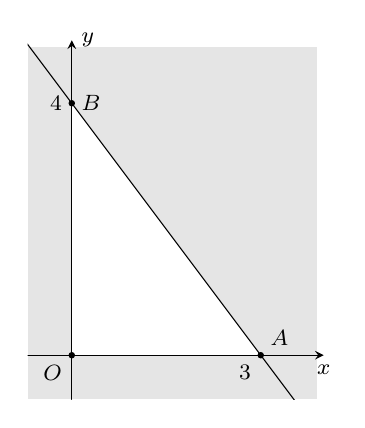
\begin{tikzpicture}[scale=.8, font=\footnotesize,line join=round, line cap=round, >=stealth];
			\clip (-0.7,-0.7) rectangle (4.2,5.2);
			\draw[color=white,fill=black!10]  (-.7,-.7) rectangle (3.9,4.9);
			\draw [color=white,fill=white](0,0)--(3,0)--(0,4)--cycle;
			\draw (3,0) node[below left]{$3$};
			\draw (0,4) node[left]{$4$};			
			\draw[->] (-0.7,0)--(4,0) node[below]{$ x $};
			\draw[->] (0,-0.7)--(0,5)	node[right]{$ y $};
			\draw (0,0) node[below left]{$O$};
			\draw[smooth,domain=-1:5] plot (\x,{-4/3*\x+4});
			\draw (3,0) node[above right]{$A$};
			\draw (0,4) node[right]{$B$};
			\draw[fill=black]  (0,0) circle (1.2pt) (3,0) circle (1.2pt) (0,4) circle (1.2pt);			
	\end{tikzpicture}}
	}
\end{ex}
%Câu 37...........................
\begin{ex}%%[0H4K2-1]%[Dự án đề kiểm tra HKII NH22-23- Tên GV]%[Mạc Đĩnh Chi]
	Tính bán kính đường tròn ngoại tiếp $\triangle A B C$ biết $A B=9, A C=15, \widehat{B A C}=120^{\circ}$.
	\choice
	{$7$}
	{\True $7\sqrt{3}$}
	{$10\sqrt{3}$}
	{$10$}
	\loigiai{
		Theo định lý cô-sin ta có\\
		$BC^2=AB^2+AC^2-2AB\cdot AC\cdot\cos\widehat{B A C}=9^2+15^2-2\cdot 9\cdot 15\cdot\dfrac{-1}{2}=441\Rightarrow BC=21$.\\
		Mặt khác $S_{ABC}=\dfrac{1}{2}\cdot AB\cdot AC\cdot \sin\widehat{B A C}=\dfrac{1}{2}\cdot 9\cdot 5\cdot \dfrac{\sqrt{3}}{2}=\dfrac{135\sqrt{3}}{4}$.\\
		Mà $S_{ABC}=\dfrac{AB\cdot AC\cdot BC}{4R}$, suy ra $\dfrac{135\sqrt{3}}{4}=\dfrac{9\cdot 15\cdot 21}{4R}\Rightarrow R=7\sqrt{3}$.
	}
\end{ex}
%Câu 38...........................
\begin{ex}%%[0D3K2-5]%[Dự án đề kiểm tra HKII NH22-23- Tên GV]%[Mạc Đĩnh Chi]
	Một công ty muốn thiết kế một loại hộp có dạng hình hộp chữ nhật có chiều cao $c=15 \mathrm{~cm}$, đáy của hình hộp chữ nhật có chu vi bằng $80 \mathrm{~cm}$. Hỏi thể tích lớn nhất của khối hộp mà công ty có thế thiết kế là bao nhiêu biết thể tích $V$ của khối hộp chữ nhật được tính bằng công thức $V=a\cdot b\cdot c$ với $a$ là chiều dài, $b$ là chiều rộng, $c$ là chiều cao?
	\choice
	{\True $6\,000 \mathrm{~cm}^3$}
	{ $5\,500 \mathrm{~cm}^3$}
	{$6\,500 \mathrm{~cm}^3$}
	{$5\,000 \mathrm{~cm}^3$}
	\loigiai{
		Gọi $x$ (cm) là chiều rộng của đáy hình hộp chữ nhật ($0<x<40$).\\
		Do đó $\left(\dfrac{80}{2}-x\right)$ (cm) là chiều dài của đáy hình hộp chữ nhật.\\
		Khi đó thể tích của hình hộp chữ nhật là\\
		$V=15(40-x)x=-15(x^2-40x)=-15(x-20)^2+6\,000\le 6\,000$, với $\forall x\in(0;40)$.\\
		Suy ra thể tích lớn nhất là $V=6\,000$ khi và chỉ khi $x=20$.\\
		Vậy thể tích lớn nhất của khối hộp mà công ty có thế thiết kế là $6\,000$ cm$^3$.
	}
\end{ex}
%Câu 39...........................
\begin{ex}%[0H4K2-1]%[Dự án đề kiểm tra HKII NH22-23- Tên GV]%[Mạc Đĩnh Chi]
	Cho tam giác $A B C$ có $A B=8, A C=12$ và $\widehat{B A C}=120^{\circ}$. Tính độ dài đường phân giác trong góc $A$ của tam giác $A B C$.
	\choice
	{$\dfrac{48}{5}$}
	{$\dfrac{48\sqrt{3}}{5}$}
	{$\dfrac{24\sqrt{3}}{5}$}
	{\True $\dfrac{24}{5}$}
	\loigiai{
		Gọi $AD$ là đường phân giác góc $A$, với $D\in BC$.\\
		Theo tính chất đường phân giác, ta có $\dfrac{DB}{DC}=\dfrac{AB}{AC}=\dfrac{8}{12}=\dfrac{2}{3}$
		\allowdisplaybreaks
		\begin{eqnarray*}
				&\Rightarrow& 3\overrightarrow{DB}=-2\overrightarrow{DC}\Rightarrow3(	\overrightarrow{AB}-\overrightarrow{AD})=-2(	\overrightarrow{AC}-\overrightarrow{AD})\\
				&\Rightarrow&\overrightarrow{AD}=\dfrac{3}{5}\overrightarrow{AB}+\dfrac{2}{5}\overrightarrow{AC}\Rightarrow\overrightarrow{AD}^2=\left(\dfrac{3}{5}\overrightarrow{AB}+\dfrac{2}{5}\overrightarrow{AC}\right)^2\\
				&\Rightarrow&AD^2=\dfrac{9}{25}AB^2+\dfrac{4}{25}AC^2+\dfrac{12}{25}AB\cdot AC\cdot\cos 120^\circ\\
				&\Rightarrow&AD^2=\dfrac{9}{25}\cdot 8^2+\dfrac{4}{25}\cdot 12^2+\dfrac{12}{25}\cdot 8\cdot 12\cdot\dfrac{-1}{2}\\
				&\Rightarrow&AD^2=\dfrac{576}{25}\Rightarrow AD=\dfrac{24}{5}.
		\end{eqnarray*}
	Vậy độ dài đường phân giác trong góc $A$ của tam giác $A B C$ là $\dfrac{24}{5}$.
	}
\end{ex}
%Câu 40...........................
\begin{ex}%%[0H4K3-1]%[Dự án đề kiểm tra HKII NH22-23- Tên GV]%[Mạc Đĩnh Chi]
	 \immini{Một tàu hàng và một tàu khách cùng xuất phát từ một vị trí ở bến tàu, đi thẳng theo hai hướng tạo với nhau một góc $60^{\circ}$. Tàu hàng chạy với tốc độ $20 \mathrm{~km} / \mathrm{h}$, tàu khách chạy với tốc độ $32 \mathrm{~km} / \mathrm{h}$. Hỏi sau 2 giờ kể từ lúc xuất phát, khoảng cách giữa hai con tàu bằng bao nhiêu km?
	\choice
	{\True $56$ km}
	{$52$ km}
	{$60$ km}
	{$49$ km}}
	{\begin{tikzpicture}[>=stealth,line join=round,line cap=round,font=\footnotesize,scale=.8]
				\path
				(0,3)coordinate (A)node[above]{\text{Bến tàu}}
				(-1,0) coordinate(B)node[below]{\text{Tàu hàng}}
				(3.5,0) coordinate(C)node[below]{\text{Tàu khách}}
				;
				\draw[->](A)--(B);
				\draw[->](A)--(C);
				\draw[fill=black]  (A) circle (1.2pt)(B) circle (1.2pt)(C) circle (1.2pt);
				\path (A) pic[draw,angle radius = 9] {angle = B--A--C} node[shift={(-75:17pt)}]{$ 60^\circ $};
		\end{tikzpicture}}
	\loigiai{
		\immini{Gọi $A$, $B$, $C$ lần lượt là vị trí bến tàu, tàu hàng và tàu khách sau $2$ giờ kể từ lúc xuất phát.\\
		Khi đó $\heva{&AB=20\cdot 2=40\\&AC=32\cdot 2=64.}$\\
		Theo định lý cô-sin trong tam giác $ABC$, ta có
		\allowdisplaybreaks
		\begin{eqnarray*}
			BC^2&=&AB^2+AC^2-2AB\cdot AC\cdot\cos 60^\circ\\
				&=&40^2+64^2-2\cdot 40\cdot 64\cdot\dfrac{1}{2}\\
				&=&3136
		\end{eqnarray*}
		$\Rightarrow BC=\sqrt{3136}=56$ km.}
	{\begin{tikzpicture}[>=stealth,line join=round,line cap=round,font=\footnotesize,scale=.8]
			\path
			(0,3)coordinate (A)node[above]{$A$}
			(-1,0) coordinate(B)node[below]{$B$}
			(3.5,0) coordinate(C)node[below]{$C$}
			;
			\draw[->](A)--(B);
			\draw[->](A)--(C);
			\draw (B)--(C);
			\draw[fill=black]  (A) circle (1.2pt)(B) circle (1.2pt)(C) circle (1.2pt);
			\path (A) pic[draw,angle radius = 9] {angle = B--A--C} node[shift={(-75:17pt)}]{$ 60^\circ $};
	\end{tikzpicture}}
	\noindent Vậy khoảng cách giữa hai con tàu sau $2$ giờ kể từ lúc xuất phát là $56$ km.
	}
\end{ex}


\Closesolutionfile{ans}
%\begin{center}
%	\textbf{ĐÁP ÁN}
%	\inputansbox{10}{ans/ans}	
%\end{center}


\begin{center}
	\textbf{PHẦN 2 - TỰ LUẬN}
\end{center}


\begin{bt}%[0T3B1-2]%[0T3B2-2]%[Dự án đề kiểm tra HKI NH22-23- Lương Như Quỳnh]%[Trường THPT Mạc Đĩnh Chi]
	\begin{enumerate}
	\item Tìm tập xác định của hàm số $ f(x)=\dfrac{x}{\sqrt{x-3}} $.
	\item Cho parabol $ (P)\colon y=x^2-mx+n $ có trục đối xứng là đường thẳng $ x=1 $. Tìm $ m $, $ n $ để parabol $ (P) $ có đỉnh $ S $ nằm trên đường thẳng $ d\colon y=4x $.
	\end{enumerate}
\loigiai{
\begin{enumerate}
	\item Hàm số $ f(x)=\dfrac{x}{\sqrt{x-3}} $ xác định khi và chỉ khi $ x-3>0 \Leftrightarrow x>3$.\\
	Vậy tập xác định của hàm số đã cho là $ \mathscr{D}=(3;+\infty) $.
	\item Trục đối xứng của parabol là đường thẳng $ x=\dfrac{-(-m)}{2\cdot 1}=1\Leftrightarrow m=2$.\\
	Đỉnh của parabol $ (P) $ là $ S(1;1-m+n) $ .\\
	Đỉnh $ S \in d\colon y=4x \Rightarrow 1-m+n=4\cdot 1 \Rightarrow n=3+m=3+2=5$.\\
	Vậy $m=2$, $n=5$ thỏa mãn yêu cầu bài toán.
	\end{enumerate}
}
\end{bt}

\begin{bt}%[0T4B1-2]%[0T5K2-5]%[Dự án đề kiểm tra HKI NH22-23- Lương Như Quỳnh]%[Trường THPT Mạc Đĩnh Chi]
	\begin{enumerate}
	\item Cho $ \sin \alpha =\dfrac{3}{4} $ với $ 90^\circ< \alpha <180^\circ $. Tính $ \cos \alpha $.
	\item Cho hình vuông $ ABCD $ cạnh bằng $ 1 $. Tính $ \left|4\overrightarrow{AB}+3\overrightarrow{AD} \right| $.
	\end{enumerate}
\loigiai{
\begin{enumerate}
	\item Ta có $ \sin ^2 \alpha +\cos ^2 \alpha=1 \Leftrightarrow \cos ^2 \alpha= 1-\sin ^2 \alpha=1-\left(\dfrac{3}{4}\right)^2=\dfrac{7}{16} \Leftrightarrow \hoac{&\cos \alpha =\dfrac{\sqrt{7}}{4}\\&\cos \alpha =-\dfrac{\sqrt{7}}{4}.}$\\
	Mà $ 90^\circ< \alpha <180^\circ \Rightarrow \cos \alpha <0 $.\\
	Vậy $ \cos \alpha =-\dfrac{\sqrt{7}} {4}$.
	\item 
	\immini{
	Ta có 
	\allowdisplaybreaks
\begin{eqnarray*}
&&  \left|4\overrightarrow{AB}+3\overrightarrow{AD} \right|^2 = \left(4\overrightarrow{AB}+3\overrightarrow{AD} \right)^2 \\ 
  &=& 16\overrightarrow{AB}^2+24 \overrightarrow{AB}\cdot \overrightarrow{AD}+9\overrightarrow{AD}^2 \\ 
    &=& 16 AB^2+9 AD^2 \text{ (Vì }AB\perp AD \text{ nên }\overrightarrow{AB}\cdot \overrightarrow{AD}=0\text{)}\\ 
    &=& 16 \cdot 1^2+9 \cdot 1^2 \\
    &=& 25.
\end{eqnarray*}
Vậy $ \left|4\overrightarrow{AB}+3\overrightarrow{AD} \right|=5 $.}
	{
	\begin{tikzpicture}
	\def\a{3}
	\path (0,0) coordinate (A)
	(0,\a) coordinate (B)
	(\a,0) coordinate (D)
	($ (B)+(D)-(A) $)coordinate (C)
	;
	\draw (A)--(B)--(C)--(D)--cycle;
	\foreach \f/\g in {A/180,B/180,D/0,C/0}{
	\draw[fill=black] (\f) circle (1pt) node[shift={(\g:7pt)},font=\scriptsize]{$ \f $};
		}	
	\end{tikzpicture}
	}
	\end{enumerate}
\immini{{\bf Cách 2}. Ta có 
	\allowdisplaybreaks
\begin{eqnarray*}
&&  4\overrightarrow{AB}+3\overrightarrow{AD} \\ &=& 3\left(\overrightarrow{AB}+\overrightarrow{AD} \right)+\overrightarrow{AB}\\ 
 &=& 3\overrightarrow{AC}+\overrightarrow{AB}
 = 3\left(\overrightarrow{AC}+\dfrac{1}{3}\overrightarrow{AB} \right)\\
 &=& 3\left(\overrightarrow{AC}+\overrightarrow{AI} \right)
 = 3\overrightarrow{AJ}.
\end{eqnarray*}
Suy ra $ \left|4\overrightarrow{AB}+3\overrightarrow{AD} \right|=\left|3\overrightarrow{AJ}\right| =3AJ$.\\
Ta có $ AJ=\sqrt{AD^2+DJ^2}=\sqrt{1^2+\left(\dfrac{4}{3}\right)^2} =\dfrac{5}{3}$.\\
Vậy $ \left|4\overrightarrow{AB}+3\overrightarrow{AD} \right|=3\cdot \dfrac{5}{3}=5 $.
}
{
	\begin{tikzpicture}
	\def\a{3}
	\path (0,0) coordinate (A)
	(0,\a) coordinate (B)
	(\a,0) coordinate (D)
	($ (B)+(D)-(A) $)coordinate (C)
	($ (A)!1/3!(B) $)coordinate (I)
	($ (D)!4/3!(C) $)coordinate (J)
	;
	\draw (A)--(B)--(C)--(D)--cycle (J)--(A)--(C)--(J)--(I);
	\foreach \f/\g in {A/180,B/180,D/0,C/0,I/180,J/0}{
	\draw[fill=black] (\f) circle (1pt) node[shift={(\g:7pt)},font=\scriptsize]{$ \f $};
		}	
	\end{tikzpicture}
}
}
\end{bt}


